\chapter {Introduction}

The freezing of a liquid into a crystalline state is the most important path to the formation of a solid. The kinetics of crystallisation play an important role in the resulting material formed by freezing, with control over the selection of crystal structure, the degree of disorder or impurities trapped during crystal growth, the shape of the grown crystal, and in some cases the failure to form a crystal at all, in favour of a glass.


The microscopic description of the freezing of molecular liquids represents both a topic of considerable interest and challenge. The mechanisms that underly the kinetics of crystallisation remain poorly understood as crystal growth kinetics are restricted to the interfacial region between the liquid and the solid phases, making the investigation of this process inaccessible by experiment. Computer simulations are a means of resolving the process through which order emerges from the liquid state. The interest, beyond a fundamental understanding of the freezing transition, stems from two lines of research. Firstly, understanding the kinetics that drive the formation of a particular crystal structure, in particular small organic drug molecules. Secondly, understanding the glass transition in organic molecules like \emph{o}-terphenyl trisnapthylbenzene and indomethiacin. Both of these approches are concerned with the properties of low temperature liquids that either promote or inhibit crystal growth.

Despite being an area of much interest, there have only been a small number of simulation studies of molecular crystallisation. A major challenge for these studies is the extremely long times required to observe crystallisation in molecular liquids compared to atomic liquids. This slow rate of crystallisation is not just a product of simulations, the experimentally determined crystal growth rates $U$ of molecular crystals are between 4 and 8 orders of magnitude slower than those of atomic crystals~\figref{growth rate}, representing one of the fundamental puzzles in our understanding of crystallisation.

\begin{figure}
    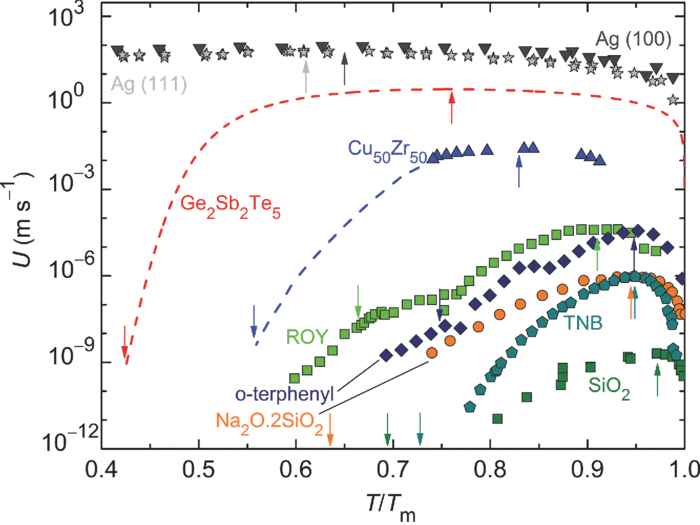
\includegraphics[width=0.7\textwidth]{growth-rate}
    \caption{Crystal growth rates relative to the melting point. The dotted lines indicate calculated values of $U$. The growth rates of molecular liquids like {\em o}-terphenyl are orders of magnitude below that on an atomic liquid like \ce{Ag}.}
    \label{growth rate}
\end{figure}

Computational modelling requires that we balance a physically realistic system with the constraints of the computational complexity of the system. If realistic molecules in 3D crystallise too slowly to be modelled by molecular dynamics simulations, perhaps we can learn something about the fundamental characteristics of crystallisation in the computationally simpler 2D system. Performing a broad analysis in 2D can identify features to later explore in a 3D system.

The goal of this project has been to i) develop tractable 2D molecules for use in simulations of liquids and crystals, ii) characterise the liquid state dynamics of these molecules, iii) identify the stable structures in the crystalline state and iv) determine the kinetics of crystallisation from supercooled molecular liquids.

This thesis is organised as follows. In \textchapref{methods} we describe the computational details of the molecular dynamics simulations. In \textchapref{dynamics} we introduce the molecular models we are using and present their dynamical behaviour in the liquid state. The determination of the stable crystal structures and the development of methods to measure crystalline order in our systems is described in \textchapref{structure}. While in \textchapref{crystallisation} we present our results on the crystallisation kinetics in our molecular systems. Through the rest of this chapter we present an introduction to the general problem of crystallisation and the behaviour of supercooled liquids.

\section{Supercooled Liquids and the Glass Transition}

The supercooled liquid phase is a metastable state formed by cooling the liquid phase below its thermodynamic freezing point. As a liquid is supercooled the structure remains almost identical to that of the liquid phase, the dynamics, however slow down dramatically. Because crystals take time to nucleate, the structural and dynamic properties of the supercooled liquid phase are important for understanding the formation of the crystal phase.

One of the characteristic features of a supercooled liquid is the dynamics. In experimental systems this is often measured as the viscosity $\rho$. We can relate the viscosity to the diffusion constant $D$, a measure of translational motion~(see \textsecref{dynamics}), by the Stokes-Einstein equation
\begin{equation}
    D = \frac{\boltzman T}{6\pi \rho r}
\end{equation}
where \boltzman is the Boltzman constant and $r$ is the radius of the particles. In the liquid state the viscosity will obey an Arrhenius type temperature dependence
\begin{equation}
    \rho = A \e^{e_A/(\boltzman T)}
\end{equation}
where $A$ is a scaling factor, $T$ is the temperature, and $e_A$ is the activation energy of the processes that comprise diffusion. Supercooled liquids however do not always adhere to this behaviour~\figref{}. Supercooled liquids that display a non-Arrhenius temperature dependence are known as \emph{fragile} liquids, with \emph{o}-terphenyl being the canonical example. As fragile liquids approach the glass transition temperature \si{\Tg}, they show a dramatic increase in the viscosity, consistent with an increasing activation energy. On the other hand \emph{strong} liquids, such as silica \ce{SiO2}, display purely Arrhenius behaviour over their entire temperature range. Liquids span the entire range of strong to weak and we characterise their fragility $m$ by their gradient at the glass transition temperature
\begin{equation}
    m = \left [ \pddiff{\log_{10}\eta}{T_g/T} \right ]
\end{equation}
where the \emph{glass transition temperature} \si{\Tg} is defined as the temperature at which the viscosity of the supercooled liquid reaches \SI{e13}{\poise}. This definition of the glass transition temperature highlights and important feature of the glass transition, it lacks a first order phase transition, instead it is a purely dynamic phase transition. Despite the lack of a first order phase transition to the glass phase, the fragility of liquids near the glass transition temperature is indicative of the glass phase being an inherent property of the liquid.

\section{Crystallisation Kinetics - Nucleation and Crystal Growth}

There are two processes that contribute to the growth of a crystal; the nucleation of an initial crystal, and the growth of that initial crystal over time. These two processes are governed by different temperature dependent properties. Nucleation is primarily a thermodynamically driven process, it is the formation of small regions of crystalline order within the liquid phase. For these regions of crystalline order to continue growing they need to be thermodynamically stable. In a system with a constant number of particles, constant pressure and constant temperature (any normal experiment carried out in a lab) the thermodynamic potential governing the system is the \emph{Gibbs free energy} $\Delta G$, with the relation 
\begin{equation}
\Delta G = \Delta H - T\Delta S
\end{equation}
where $\Delta H$ is the change in enthalpy, $\Delta S$ is the change in entropy and $T$ is the temperature. At the melting point, both the liquid surrounding a crystal nucleus and the crystal structure inside the crystal nucleus have the same energy however there is a free energy cost to the boundary between the two regions making the crystal nucleus unstable. By reducing the temperature below the melting point the additional entropy of the liquid phase gives it a larger free energy than the crystal phase. As we reduce the temperature the extra free energy of the crystal phase makes up for the free energy cost of the boundary stabilising the nucleus. In experimental crystal growth rates~\figref{} we see the stabilisation of the crystal nucleus increase the growth rate until the kinetics, the second contributor to the growth rate of a crystal, limits the growth of the crystal. For crystal growth to occur molecules need to rearrange to align both position and orientation with the existing crystal region. At low temperatures the dynamics of these processes become slow and limit the crystal growth.

The dynamics of the crystal growth are also interesting for its anisotropy. All crystal growth has some preferred directions, otherwise crystals would be spherical. In its simplest form anisotropic growth occurs when molecules will preferentially attach at a step boundary~\figref{} in existing structures. In more complicated crystal structures like rods, it is growth occurring preferentially in some directions that leads to these shapes.


\section{Aims of this Project}

This project aims to provide insight into the effect that molecular shape has on the dynamics of the crystal-liquid phase transition. To understand this transition we first need to investigate how shape affects the dynamics properties of the liquid phase and the structural properties of the crystal phase.
